\section{Results}\label{results}

\subsection{Run integrity and panel scale}

The full diagnostic-reference panel completed 144 annual EnergyPlus cases. Each trace contains 35{,}040 records and 16{,}704 occupied probability records, yielding 2{,}405{,}376 occupied records. The trace schema was consistent across cases, all 45 raw zone environmental fields were populated during occupied periods, and no fatal EnergyPlus errors occurred. Sixteen cases reported warmup-convergence Severe messages, but EnergyPlus completed successfully in each case. These messages are treated as simulation QA limitations rather than failed cases.

Because the diagnostic-reference strategy did not use the probability outputs to adjust setpoints, the results below describe representation behavior under fixed simulated environments. They should not be read as closed-loop HVAC outcomes.

\subsection{Mean TSV and discomfort-tail probability}

Across the full panel, mean $p_{\mathrm{tail}}$ was 0.117 and the 95th percentile was 0.306. Using the screening cutoff $p_{\mathrm{tail}}\ge0.20$, 13.4\% of occupied records were high-tail states. High-tail exceedance increased with later time slices and higher scenario forcing (Table~\ref{tab:panel_tail_summary}). The baseline-2020s slice had 9.17\% high-tail exceedance, while the late-2080s slice had 21.18\%. SSP2-4.5 had 11.75\% high-tail exceedance, while SSP5-8.5 had 15.15\%.

\begin{table}[htbp]
\centering
\caption{High-tail exceedance summary for the 144-case fixed-reference panel. High-tail exceedance is the share of occupied records with $p_{\mathrm{tail}}\ge0.20$.}
\label{tab:panel_tail_summary}
\footnotesize
\begin{tabular}{llrr}
\toprule
\textbf{Grouping} & \textbf{Level} & \textbf{Mean $p_{\mathrm{tail}}$} & \textbf{High-tail exceedance (\%)} \\
\midrule
All & Full panel & 0.117 & 13.45 \\
\midrule
Scenario & SSP2-4.5 & 0.112 & 11.75 \\
Scenario & SSP5-8.5 & 0.121 & 15.15 \\
\midrule
Time slice & baseline\_2020s & 0.105 & 9.17 \\
Time slice & near\_2030s & 0.105 & 9.16 \\
Time slice & mid\_2050s & 0.118 & 14.28 \\
Time slice & late\_2080s & 0.137 & 21.18 \\
\midrule
Severity & typical & 0.109 & 10.48 \\
Severity & hot & 0.120 & 14.79 \\
Severity & heatwave\_extreme & 0.121 & 15.07 \\
\bottomrule
\end{tabular}
\end{table}

City differences were large. Kolkata had the highest mean-zone high-tail exceedance (19.90\%), followed by Ahmedabad (17.11\%), Phoenix (13.36\%), Guangzhou (12.51\%), Houston (12.33\%), and Beijing (5.48\%). The highest case-level exceedance rates occurred in hot or heatwave-extreme late-century files, including Kolkata SSP5-8.5 late-2080s hot and heatwave-extreme cases, both at 41.13\% high-tail exceedance.

\begin{figure}[H]
    \centering
    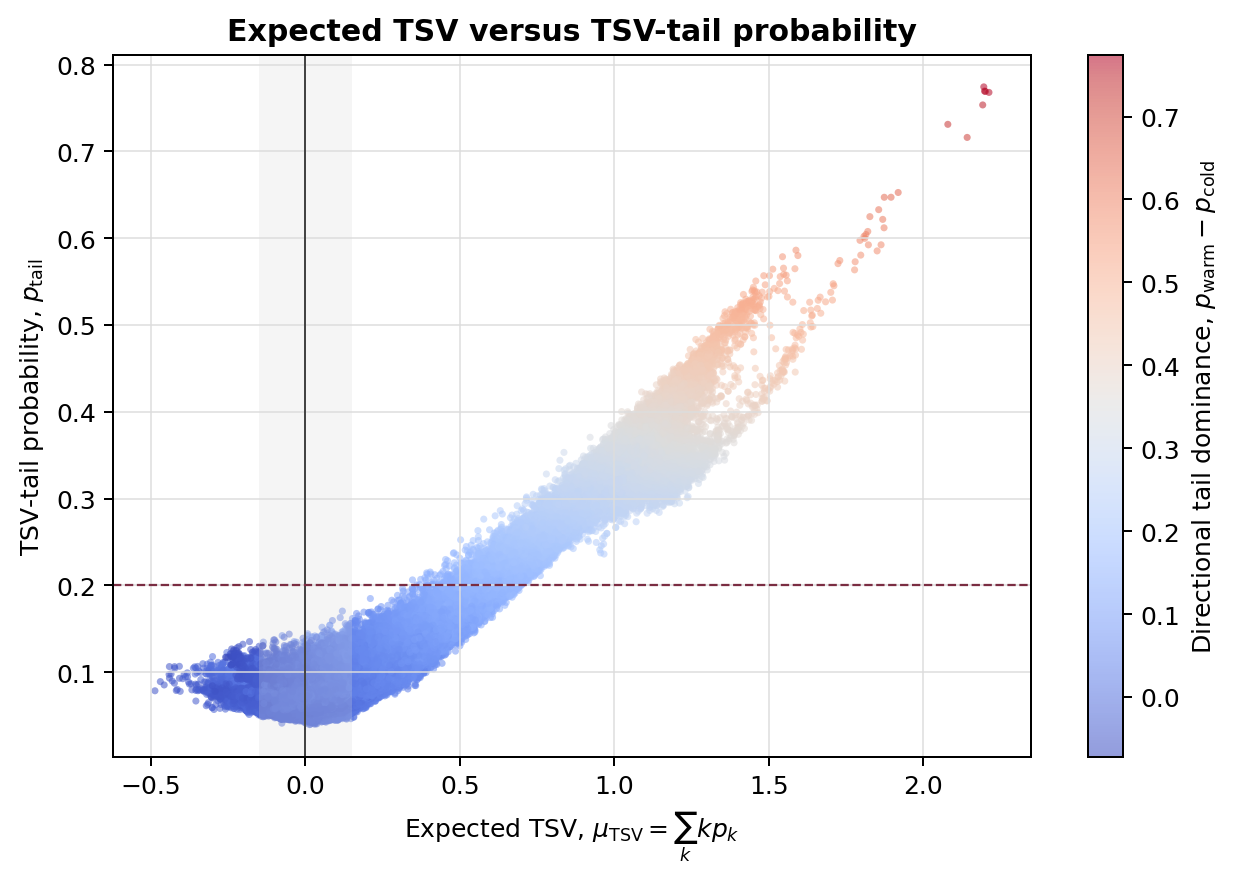
\includegraphics[width=0.86\linewidth]{figs/mean_vs_tail_scatter_sample.png}
    \caption{Expected TSV versus discomfort-tail probability for a sampled subset of the 144-case diagnostic panel. Expected TSV denotes the probability-weighted mean $\mu_{\mathrm{TSV}}=\sum_k k p_k$, not the most likely TSV class. The horizontal line marks the screening cutoff $p_{\mathrm{tail}}=0.20$. Expected TSV is informative, but $p_{\mathrm{tail}}$ is the quantity that directly encodes the selected high-tail flag.}
    \label{fig:mean_tail_scatter}
\end{figure}

Figure~\ref{fig:mean_tail_scatter} shows the internal relationship between the TSV probability distribution and two summaries derived from it. Expected TSV remained strongly associated with discomfort-tail probability, so the scalar mean is not meaningless. The diagnostic does not show near-neutral high-tail states under the strict condition $|\mu_{\mathrm{TSV}}|<0.15$; that share was 0.0\%. The stronger finding is different: similar positive mean states can still carry materially different tail probabilities. In the same-mean contrast examples, pairs with nearly equal $\mu_{\mathrm{TSV}}$ differed in $p_{\mathrm{tail}}$ by up to about 0.18. For example, late-century Kolkata and Phoenix records with $\mu_{\mathrm{TSV}}\approx1.35$ had $p_{\mathrm{tail}}$ values of 0.340 and 0.518, respectively. A scalar mean gives the warm-side tendency, but the probability distribution shows how much mass has accumulated in the severe tail.

The same figure also shows that tail risk in this fixed-reference panel is warm-dominant. Mean warm-tail probability was 0.089, compared with 0.027 for the cold tail. Warm-tail probability exceeded cold-tail probability in 78.9\% of occupied records and in all records crossing $p_{\mathrm{tail}}\ge0.20$. Records with $\mu_{\mathrm{TSV}}\le0$ never crossed the high-tail screen, while all records with $\mu_{\mathrm{TSV}}>1$ did. Thus, above about $+1$ expected TSV, the scalar mean already identifies a warm-risk state; the probability distribution is still needed to quantify how much severe-tail mass is present.

\subsection{PMV as a scalar benchmark}

The PMV comparison gives a second scalar benchmark. Across the same occupied records, $|\mathrm{PMV}|$ was correlated with $p_{\mathrm{tail}}$ (Pearson $r=0.856$, Spearman $\rho=0.751$), while $|\mu_{\mathrm{TSV}}|$ was more tightly correlated with $p_{\mathrm{tail}}$ (Pearson $r=0.976$, Spearman $\rho=0.896$). A best offline $|\mu_{\mathrm{TSV}}|$ threshold of 0.609 disagreed with the high-tail flag in 1.09\% of occupied records. A best offline $|\mathrm{PMV}|$ threshold of 0.912 disagreed in 3.37\% of occupied records.

\begin{figure}[H]
    \centering
    
\includegraphics[width=\linewidth]{figs/scalar_tail_comparison_hexbin.png}
    \caption{Scalar comparison against the primary TSV probability output. Left: $|\mu_{\mathrm{TSV}}|$ versus $p_{\mathrm{tail}}$. Right: $|\mathrm{PMV}|$ versus the same $p_{\mathrm{tail}}$ distribution. Both panels use the same 0--3 scalar range. The vertical line marks the conventional 0.5 scalar band, and the horizontal line marks the diagnostic high-tail screen $p_{\mathrm{tail}}=0.20$.}
    \label{fig:pmv_scalar_comparison}
\end{figure}

\begin{table}[htbp]
\centering
\caption{Scalar threshold comparison against the $p_{\mathrm{tail}}\ge0.20$ high-tail flag. Best thresholds are optimized offline over the full diagnostic panel. Missed high-tail and false-positive rates are reported as percentages of all occupied records.}
\label{tab:pmv_scalar_comparison}
\scriptsize
\resizebox{\textwidth}{!}{%
\begin{tabular}{lrrrr}
\toprule
\textbf{Scalar rule} & \textbf{Threshold} & \textbf{Disagreement (\%)} & \textbf{Missed high-tail (\% records)} & \textbf{False positive (\% records)} \\
\midrule
$|\mu_{\mathrm{TSV}}|$ best threshold & 0.609 & 1.09 & 0.62 & 0.47 \\
$|\mathrm{PMV}|$ best threshold & 0.912 & 3.37 & 1.56 & 1.81 \\
$|\mathrm{PMV}|$ standard band & 0.500 & 19.11 & 0.006 & 19.10 \\
\bottomrule
\end{tabular}
}
\end{table}

Read together, Figures~\ref{fig:mean_tail_scatter} and~\ref{fig:pmv_scalar_comparison} separate two issues. Figure~\ref{fig:mean_tail_scatter} shows how the learned TSV expectation relates to its own tail probability. Figure~\ref{fig:pmv_scalar_comparison} asks how that relationship differs from PMV, Fanger's continuous comfort index built from thermal-balance terms and empirical chamber-vote evidence. The standard $|\mathrm{PMV}|=0.5$ band behaved conservatively in this panel. It almost never missed high-tail states, but it flagged many states that did not cross $p_{\mathrm{tail}}\ge0.20$. The learned expected-TSV scalar occupies a narrower range and follows the calibrated tail probability closely because both are summaries of the same seven-class probability vector. This is a tighter empirical association, not a claim of linearity: $|\mu_{\mathrm{TSV}}|$ reports the location of the predicted distribution, while $p_{\mathrm{tail}}$ reports its severe-category mass. Its maximum absolute value was 2.24 in this panel, and only 3.7\% of occupied records exceeded $|\mu_{\mathrm{TSV}}|=1$. PMV spans a wider scalar range, reaching 3.31 in absolute value, and includes a lower-$p_{\mathrm{tail}}$ branch at higher $|\mathrm{PMV}|$ values. This broad branch around $p_{\mathrm{tail}}\approx0.1$ is the visual source of the conservative PMV result: PMV can assign a large scalar departure to states that the calibrated TSV distribution still places mostly in neutral or mild categories. Among records with $|\mathrm{PMV}|\ge0.5$, 58.7\% remained below $p_{\mathrm{tail}}=0.20$; even among records with $|\mathrm{PMV}|\ge1$, 9.6\% remained below that tail-probability screen. The mid-tail band shows the same compression: for records with $0.3\le p_{\mathrm{tail}}<0.4$, the 5th--95th percentile range was 0.88--1.20 for $|\mu_{\mathrm{TSV}}|$ but 1.04--1.86 for $|\mathrm{PMV}|$. The point is not that PMV is useless or blind to thermal stress; rather, PMV and $p_{\mathrm{tail}}$ answer different diagnostic questions. PMV gives a conventional continuous mean-vote index for the thermal state. $p_{\mathrm{tail}}$ reports the predicted probability mass in severe TSV categories.

The no-PMV robustness check gave the same qualitative result, but it should be read as a model-output comparison rather than as two versions of PMV. Figure~\ref{fig:pmv_feature_robustness} keeps the x-axis fixed as the same stored $|\mathrm{PMV}|$ scalar and changes the y-axis from the primary $p_{\mathrm{tail}}$ output to the $p_{\mathrm{tail}}$ output from a separately trained no-PMV TSV predictor. Removing PMV from the ordinal predictor changed the mean-zone high-tail exceedance at $p_{\mathrm{tail}}\ge0.20$ from 13.45\% to 13.85\%, and changed any-zone exceedance from 37.03\% to 37.52\%. The PMV-inclusive output is modestly tighter against the PMV scalar, with Pearson $r=0.856$ and Spearman $\rho=0.751$, compared with $r=0.849$ and $\rho=0.726$ for the no-PMV output. This supports a limited interpretation: calculable PMV is a useful predictor feature for reported TSV probabilities, but the main scalar-reference and aggregation results are not created solely by including PMV in the model. Under the no-PMV predictor, $|\mu_{\mathrm{TSV}}|$ still had Pearson $r=0.976$ with its own $p_{\mathrm{tail}}$ output. We therefore treat the PMV comparison as a descriptive scalar-reference audit, not as the main evidence for the probability diagnostic.

\begin{figure}[htbp]
    \centering
    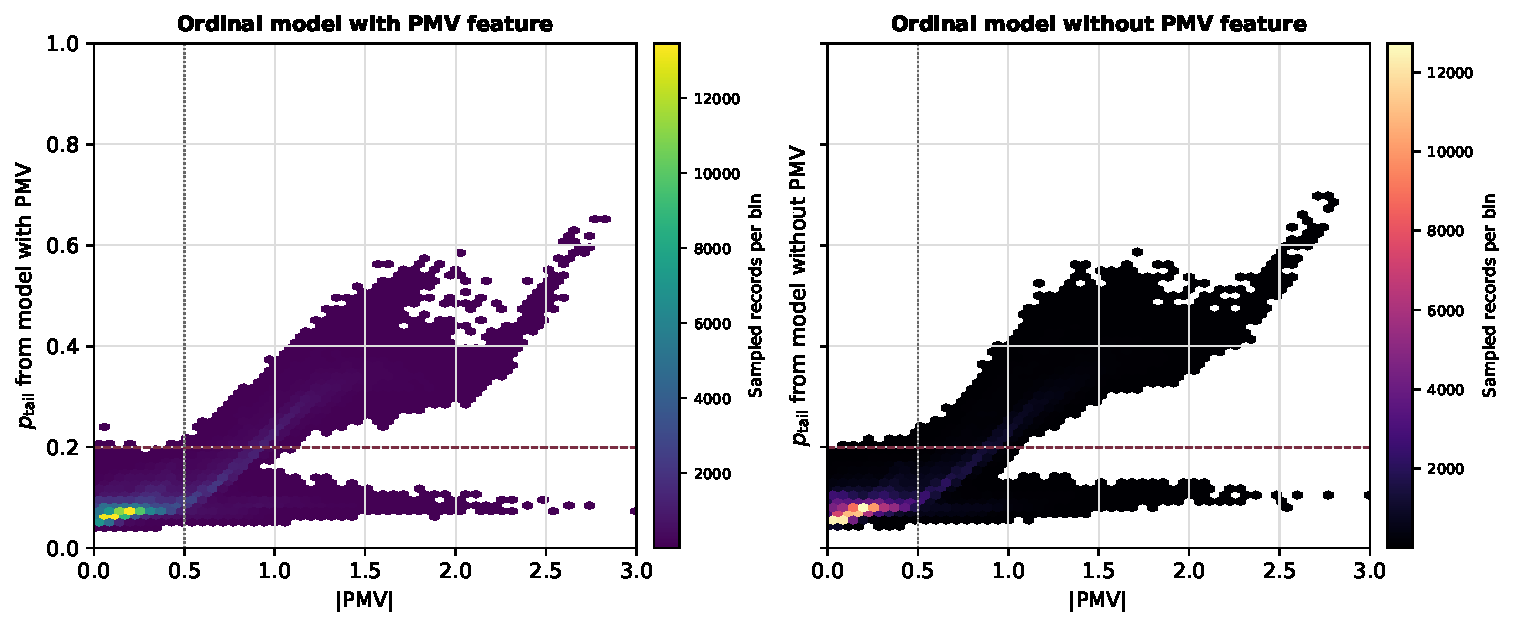
\includegraphics[width=\linewidth]{figs/pmv_feature_robustness_hexbin.pdf}
    \caption{PMV-scalar robustness check using two TSV probability outputs. Both panels use the same x-axis scalar, $|\mathrm{PMV}|$, from the simulated thermal state. The left panel plots PMV against $p_{\mathrm{tail}}$ from the primary TSV predictor, which includes PMV as an engineered covariate. The right panel plots the same PMV values against $p_{\mathrm{tail}}$ from a separately trained no-PMV TSV predictor. The different palettes indicate that the two panels contain different probability-model outputs, not different PMV calculations.}
    \label{fig:pmv_feature_robustness}
\end{figure}

The held-out TSV validation check gives the same practical reading (Tables~\ref{tab:tail_probability_comparison} and~\ref{tab:tsv_predictor_validation}). The primary TSV predictor was slightly stronger than the no-PMV predictor, but the difference was small: exact-class accuracy changed from 47.3\% to 46.9\%, within-one-class accuracy from 84.1\% to 83.8\%, and ordinal class MAE from 0.73 to 0.73. The rounded-PMV class baseline was weaker on exact and ordinal metrics, with 33.2\% exact accuracy and 0.97 class MAE. Class-specific recall was modest in the tail classes for all methods, which is consistent with the neutral-heavy and noisy structure of field TSV data. Supplementary calibration checks show that aggregate predicted $p_{\mathrm{tail}}$ aligned closely with observed tail frequency on the held-out split: the primary model's mean predicted $p_{\mathrm{tail}}$ was 0.207 versus an observed tail frequency of 0.206, with fixed-bin tail ECE of 0.011. We also tested a PMV-only calibrated tail baseline, fitted as $|\mathrm{PMV}|\rightarrow\Pr(\mathrm{TSV}\le-2\ \mathrm{or}\ \mathrm{TSV}\ge+2)$ on the same non-test data. Table~\ref{tab:tail_probability_comparison} shows that this baseline matched overall tail prevalence on the held-out split, but it discriminated tail records less well than the TSV probability models. AUROC was 0.571 versus 0.747, average precision was 0.260 versus 0.483--0.487, Brier score was 0.161 versus 0.137--0.138, and F1 at the $p_{\mathrm{tail}}\ge0.20$ screen was 32.6\% versus 46.4--47.1\%. A stricter contributor-grouped robustness check in the supplement showed weaker transfer, especially for tail-class discrimination, which limits any absolute reading of simulated tail-risk percentages under domain shift. It also showed only small differences between the primary and no-PMV feature sets. The validation evidence therefore supports a limited claim: PMV is useful enough to improve the primary ordinal predictor slightly, and PMV alone can be calibrated to the overall tail prevalence, but the 144-case diagnostic patterns should not be treated as a PMV-only artifact.

\begin{table}[htbp]
\centering
\caption{Held-out tail-probability comparison for the TSV probability models and the PMV-only calibrated scalar baseline. F1 is computed by screening each predicted tail probability at $p_{\mathrm{tail}}\ge0.20$.}
\label{tab:tail_probability_comparison}
\scriptsize
\setlength{\tabcolsep}{4.2pt}
\begin{tabular}{lrrrrrr}
\toprule
\textbf{Predictor} & \textbf{Mean predicted} & \textbf{Observed} & \textbf{Brier} & \textbf{ECE} & \textbf{F1 (\%)} & \textbf{AUROC} \\
\midrule
Primary TSV model & 0.207 & 0.206 & 0.137 & 0.011 & 47.1 & 0.747 \\
No-PMV TSV model & 0.207 & 0.206 & 0.138 & 0.006 & 46.4 & 0.747 \\
PMV-only calibrated tail baseline & 0.206 & 0.206 & 0.161 & 0.003 & 32.6 & 0.571 \\
\bottomrule
\end{tabular}
\end{table}

\begin{table}[htbp]
\centering
\caption{Held-out TSV class validation for the primary predictor, the no-PMV robustness predictor, and a rounded-PMV class baseline. The PMV baseline rounds PMV to the nearest TSV class and clips to $[-3,+3]$; it is a deterministic scalar-label baseline, not a probability model. Class recall columns report the share of records in each observed TSV class assigned to that same class.}
\label{tab:tsv_predictor_validation}
\scriptsize
\resizebox{\textwidth}{!}{%
\begin{tabular}{lrrrrrrrrrrrr}
\toprule
\textbf{Predictor} & \textbf{Exact (\%)} & \textbf{Within $\pm1$ (\%)} & \textbf{Class MAE} & \textbf{Tail F1 (\%)} & \textbf{Log loss} & \textbf{TSV -3} & \textbf{TSV -2} & \textbf{TSV -1} & \textbf{TSV 0} & \textbf{TSV +1} & \textbf{TSV +2} & \textbf{TSV +3} \\
\midrule
Primary TSV model & 47.3 & 84.1 & 0.73 & 34.0 & 1.454 & 25.5 & 6.9 & 12.4 & 88.0 & 16.2 & 15.7 & 23.9 \\
No-PMV TSV model & 46.9 & 83.8 & 0.73 & 33.5 & 1.476 & 23.7 & 6.5 & 13.0 & 87.4 & 15.4 & 15.8 & 23.2 \\
Rounded PMV class & 33.2 & 76.5 & 0.97 & 26.6 & -- & 13.8 & 10.4 & 27.6 & 47.8 & 26.3 & 14.5 & 10.5 \\
\bottomrule
\end{tabular}
}
\end{table}

\subsection{Zone aggregation hides any-zone tail exceedance}

Mean-zone aggregation produced a stable building-level summary, but it also hid zone-level risk. Across the full panel, mean-zone aggregation identified 13.45\% high-tail exceedance. Any-zone aggregation identified 37.03\%, and p90-zone aggregation identified 28.19\%. These are modeled occupied-timestep zone-state exceedances, not measured occupant exposures. In 23.58\% of occupied records, the mean-zone value was below $p_{\mathrm{tail}}=0.20$ while at least one zone exceeded it. A maximum-zone summary would assign a more severe tail category than the mean in 31.69\% of occupied records; a p90-zone summary would do so in 20.94\%.

The area-weighted zone-time diagnostic gives a useful check on this result. When each zone-time record was weighted by conditioned floor area, high-tail exceedance was 13.17\%, close to the mean-zone value. This does not remove the local risk signal. It shows that much of the hidden any-zone exceedance comes from smaller perimeter zones rather than from the largest core zones.

The aggregation result is not an artifact of choosing 0.20 as the reporting screen. Figure~\ref{fig:tail_threshold_sensitivity} repeats the exceedance calculation from $\tau=0.05$ to $\tau=0.40$, where $\tau$ is the high-tail screen applied to $p_{\mathrm{tail}}$. Absolute exceedance falls as the screen becomes stricter, but any-zone exceedance remains well above mean-zone exceedance across the range. For example, at $\tau=0.10$, mean-zone exceedance was 35.74\% and any-zone exceedance was 60.78\%; at $\tau=0.30$, they were 5.46\% and 24.10\%, respectively. Hidden any-zone exceedance remained between 18.63\% and 25.32\% for thresholds from 0.10 to 0.30. The no-PMV predictor showed the same pattern: at $\tau=0.20$, mean-zone exceedance was 13.85\%, any-zone exceedance was 37.52\%, and hidden any-zone exceedance was 23.67\%.

\begin{figure}[htbp]
    \centering
    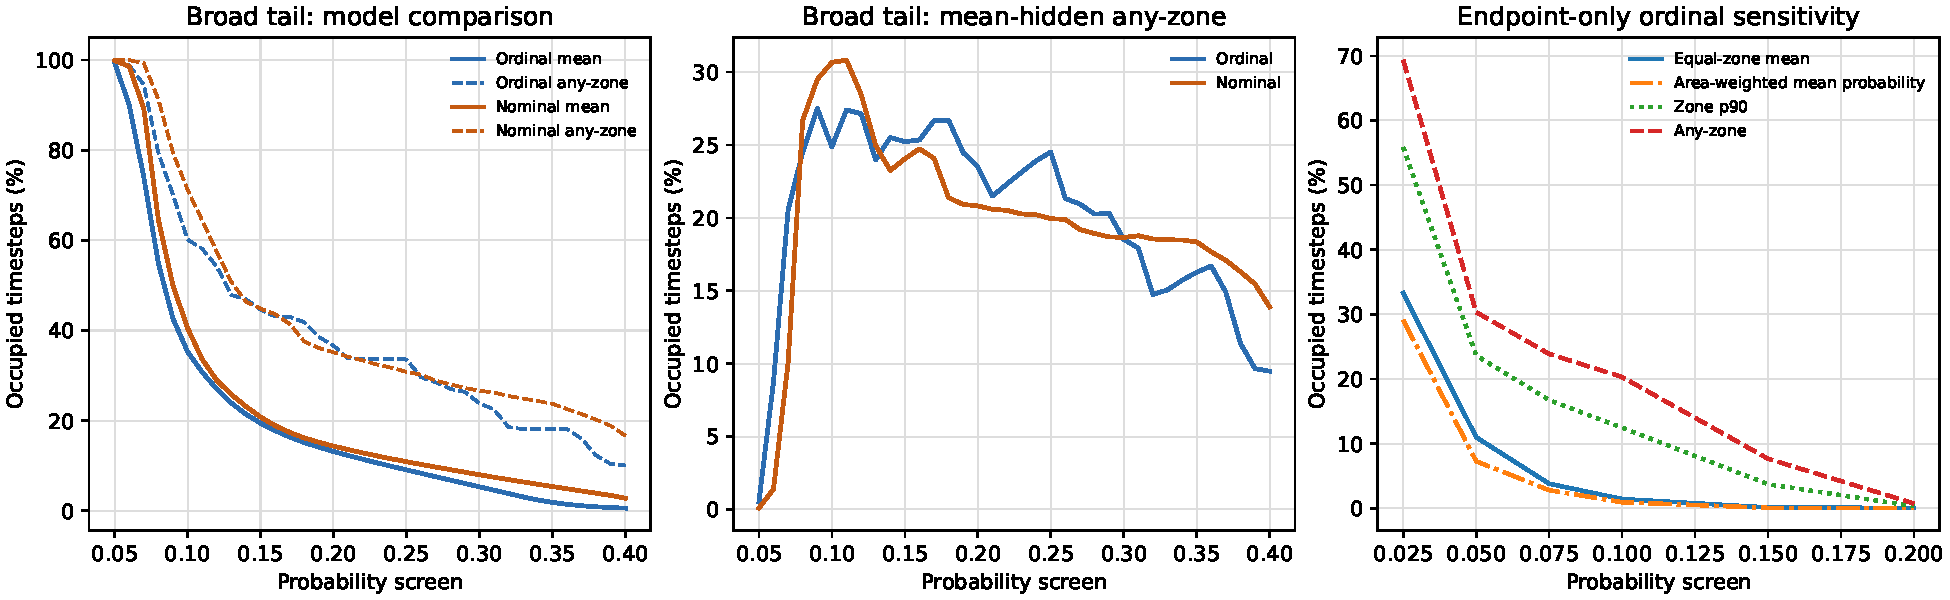
\includegraphics[width=0.82\linewidth]{figs/p_tail_threshold_sensitivity.pdf}
    \caption{Sensitivity of high-tail exceedance to the selected $p_{\mathrm{tail}}$ screen. The vertical line marks the manuscript reporting screen $\tau=0.20$. The persistent gap between mean-zone, p90-zone, and any-zone exceedance shows that the zone-aggregation result is not specific to a single threshold.}
    \label{fig:tail_threshold_sensitivity}
\end{figure}

\begin{table}[htbp]
\centering
\caption{Zone aggregation summary by city. Mean, any-zone, and p90-zone columns report modeled high-tail exceedance at $p_{\mathrm{tail}}\ge0.20$. Any-zone exceedance is the share of occupied timesteps for which the maximum zone value satisfies $\max_z p_{\mathrm{tail},z}\ge0.20$. Hidden high-tail exceedance means the mean-zone value is below 0.20 while at least one zone is at or above 0.20.}
\label{tab:zone_aggregation_summary}
\scriptsize
\resizebox{\textwidth}{!}{%
\begin{tabular}{lrrrrr}
\toprule
\textbf{City} & \textbf{Mean-zone (\%)} & \textbf{Area-weighted zone-time (\%)} & \textbf{Any-zone (\%)} & \textbf{p90-zone (\%)} & \textbf{Hidden any-zone (\%)} \\
\midrule
Ahmedabad & 17.11 & 17.66 & 54.48 & 42.16 & 37.37 \\
Beijing & 5.48 & 5.86 & 15.55 & 9.98 & 10.07 \\
Guangzhou & 12.51 & 11.92 & 32.08 & 23.27 & 19.56 \\
Houston & 12.33 & 11.06 & 28.18 & 22.31 & 15.85 \\
Kolkata & 19.90 & 20.73 & 47.27 & 36.36 & 27.36 \\
Phoenix & 13.36 & 11.81 & 44.64 & 35.07 & 31.28 \\
\bottomrule
\end{tabular}
}
\end{table}

The highest-risk zones were perimeter zones, especially P1, the south perimeter orientation in this DOE Medium Office geometry. The largest high-tail exceedance rates were 30.51\% for \texttt{perimeter\_bot\_zn\_1}, 27.91\% for \texttt{perimeter\_mid\_zn\_1}, and 23.59\% for \texttt{perimeter\_top\_zn\_1}. Each of these zones accounts for about 4.16\% of conditioned floor area, while each core zone accounts for about 19.74\%. Thus, the most severe modeled local tail exceedance occurs in relatively small perimeter zones, while the building-level area-weighted signal is shaped strongly by the larger core zones.

Figure~\ref{fig:zone_size_mosaic} shows that this local pattern changes by city and time slice. Beijing remains comparatively low-risk across the panel: its maximum zone-mean high-tail exceedance rises from 8.8\% in the baseline-2020s slice to 18.6\% in the late-2080s slice. Guangzhou shows a clearer future-weather transition, with the maximum zone value increasing from 23.1\% in the baseline-2020s slice to 34.3\% in the mid-2050s slice and 53.1\% in the late-2080s slice. Kolkata reaches high exceedance earlier: its maximum zone value is already 39.2\% in the baseline-2020s slice and reaches 65.0\% in the mid-2050s slice. Ahmedabad has a different structure: P1 is already highly exposed, but non-P1 perimeter and core zones remain much lower until the late-2080s slice. This is why Ahmedabad can look severe under an any-zone view while the broader zone field is less uniformly severe than Kolkata.

\begin{figure}[p]
    \centering
    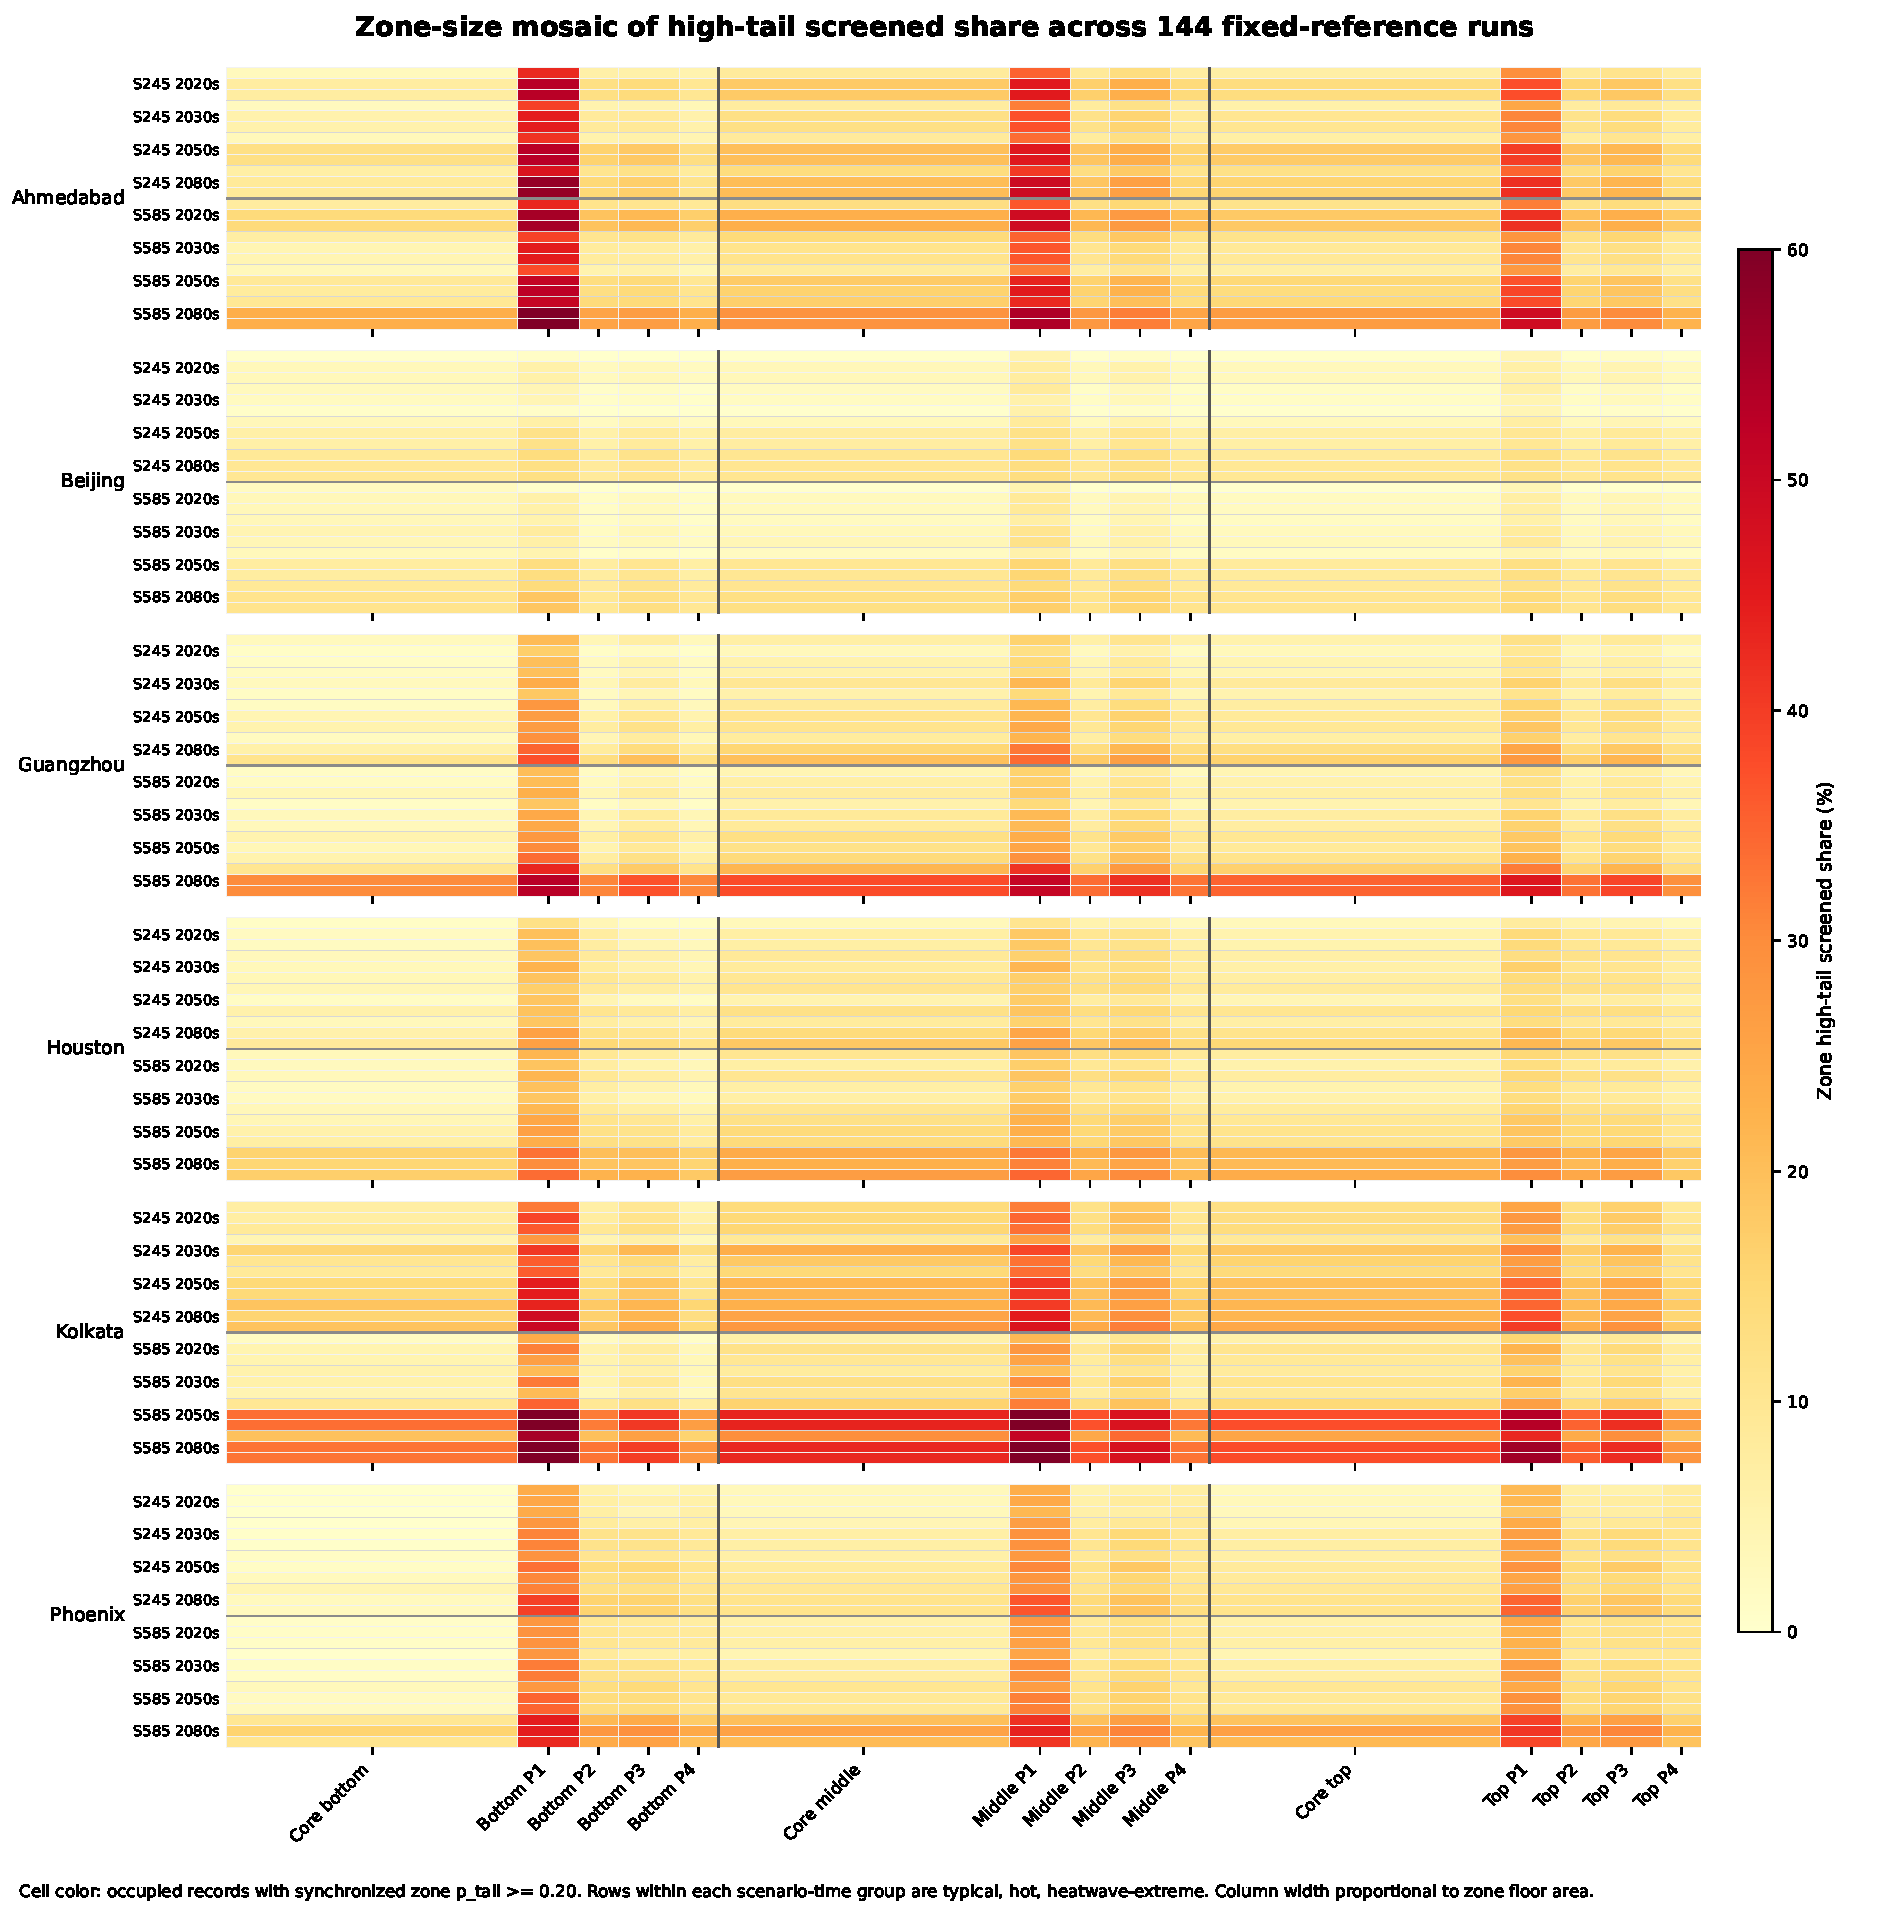
\includegraphics[width=\linewidth,height=0.86\textheight,keepaspectratio]{figs/zone_size_mosaic_heatmap_area.pdf}
    \caption{Zone-size mosaic of modeled high-tail exceedance across the 144-case fixed-reference panel. Cell color reports the share of occupied records in each case-zone pair with $p_{\mathrm{tail}}\ge0.20$. Column width is proportional to conditioned floor area, so the figure compares local tail exceedance with the physical size of the zone carrying that signal. Core bottom, core middle, and core top are the three core zones of the DOE Medium Office prototype; Bottom P1--P4, Middle P1--P4, and Top P1--P4 are the four perimeter zones on each floor level. P1--P4 denote perimeter orientations: P1 south, P2 east, P3 north, and P4 west. The conditioned top zones sit below the top-floor plenum and roof assembly, so ``top'' should not be read as a directly roof-exposed room condition. Rows within each scenario-time group are ordered as typical, hot, and heatwave-extreme weather files.}
    \label{fig:zone_size_mosaic}
\end{figure}

Figure~\ref{fig:zone_floor_position} was generated as a direct check on the floor/orientation reading from Fig.~\ref{fig:zone_size_mosaic}. It prevents over-reading the mosaic as a simple floor-height effect. Area-weighted high-tail exceedance was 11.04\% for the bottom floor, 15.11\% for the middle floor, and 13.36\% for the top floor. The middle floor had the highest area-weighted floor exceedance in 135 of 144 cases. Bottom-floor exceedance was highest only under an any-zone-within-floor summary, where the south perimeter zone P1 dominated. Bottom P1 had 30.51\% high-tail exceedance, compared with 27.91\% for middle P1 and 23.59\% for top P1. For the other perimeter orientations, bottom was not the highest. We therefore interpret the floor pattern as a prototype-specific interaction between perimeter orientation, floor construction, and zone conditioning, not as a general result that lower floors are more exposed than upper floors. High-tail states were warm-dominant in all zones under the $p_{\mathrm{tail}}\ge0.20$ screen.

\begin{figure}[htbp]
    \centering
    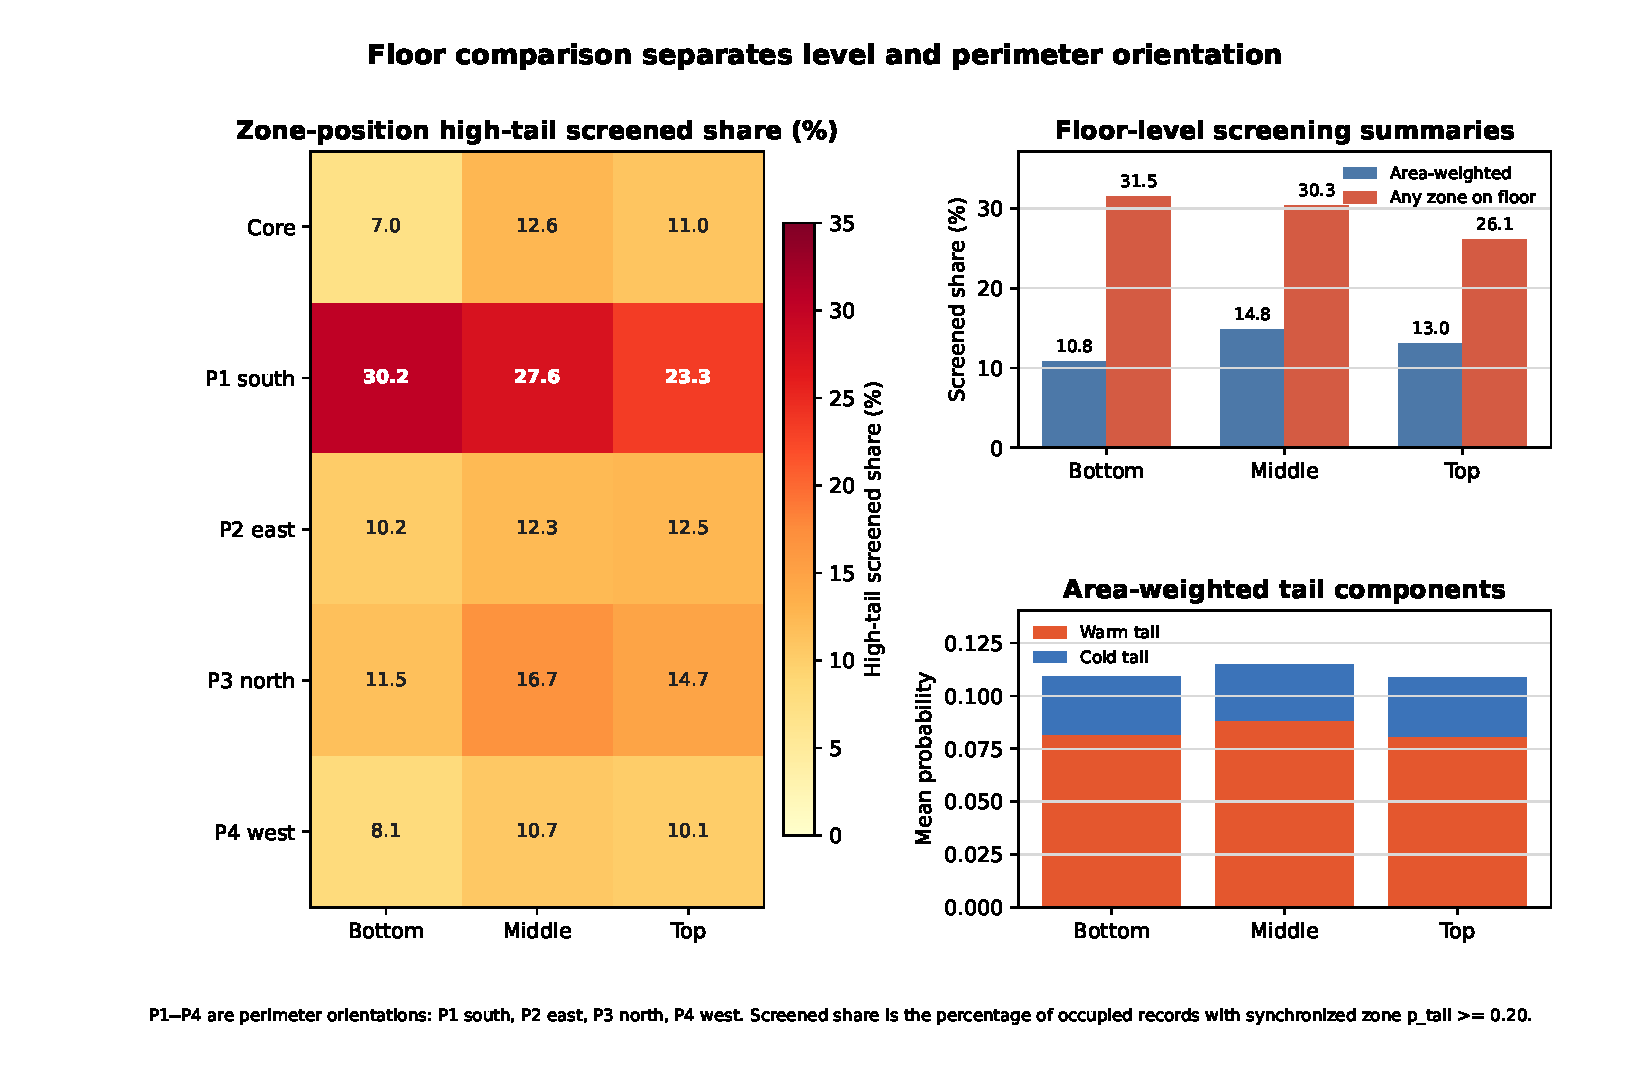
\includegraphics[width=\linewidth]{figs/zone_floor_position_comparison.pdf}
    \caption{Floor-position comparison for the 144-case fixed-reference panel. The heat map reports modeled high-tail exceedance by floor and zone position. P1--P4 are the perimeter orientations in the DOE Medium Office prototype: P1 south, P2 east, P3 north, and P4 west. Area-weighted floor exceedance summarizes zone-time records using conditioned floor area, while any-zone floor exceedance reports the share of occupied records in which at least one zone on that floor exceeds $p_{\mathrm{tail}}\ge0.20$. Tail-component bars show that floor differences are driven mainly by the warm tail.}
    \label{fig:zone_floor_position}
\end{figure}

\subsection{Metabolic-spread sensitivity}

The metabolic-spread diagnostic shows that representative occupant assumptions can materially change the tail-risk profile even when the simulated thermal environments are held fixed. Across 216{,}483{,}840 zone-profile probability evaluations, the mean spread in mean-zone $p_{\mathrm{tail}}$ across the six metabolic profiles was 0.074, with a 95th percentile spread of 0.209. For max-zone $p_{\mathrm{tail}}$, the mean spread was 0.137 and the 95th percentile spread was 0.327.

Changing the metabolic profile also changed threshold status. Mean-zone high-tail status flipped across metabolic profiles in 18.99\% of occupied records, and max-zone high-tail status flipped in 38.66\%. When the S-real profile remained below the high-tail cutoff, some other metabolic profile crossed it in 18.80\% of mean-zone records and 36.51\% of any-zone records. Because the fixed-reference panel is warm-tail dominated, lower metabolic-load profiles generally reduced predicted high-tail exposure. In this diagnostic, a lower metabolic input means the same simulated thermal environment is interpreted by the reported-TSV model with less occupant metabolic heat.

\begin{table}[htbp]
\centering
\caption{Scenario-level metabolic-spread results. Values are recomputed over fixed environmental traces; EnergyPlus was not rerun with altered occupant heat gains.}
\label{tab:metabolic_scenario_summary}
\footnotesize
\begin{tabular}{lrrrr}
\toprule
\textbf{Profile} & \textbf{W/person} & \textbf{met} & \textbf{Mean-zone high-tail (\%)} & \textbf{Any-zone high-tail (\%)} \\
\midrule
COMP-Lo & 90.0 & 0.900 & 3.32 & 13.82 \\
S-real & 93.2 & 0.932 & 3.10 & 14.89 \\
COMP-Med & 100.0 & 1.000 & 7.97 & 29.78 \\
EQ-Max & 108.0 & 1.080 & 21.20 & 45.37 \\
COMP-Hi & 110.0 & 1.100 & 13.66 & 38.44 \\
LEGACY & 120.0 & 1.200 & 17.32 & 47.87 \\
\bottomrule
\end{tabular}
\end{table}

The response is not strictly monotone across all adjacent profiles; in particular, the calibrated model gives lower mean-zone high-tail exposure at 110 W/person than at 108 W/person. We therefore interpret this section as a sensitivity diagnostic across metabolic assumptions, not as a smooth physiological dose-response curve. The practical result is still clear: the single representative occupant assumption can hide a substantial range of predicted reported-TSV tail exposure.

The zone-resolved profile summaries show where this sensitivity is concentrated. Across the 2{,}160 case-zone summaries for each profile, mean case-zone high-tail exposure was 3.27\% for COMP-Lo, 3.26\% for S-real, 8.65\% for COMP-Med, 19.25\% for EQ-Max, 15.37\% for COMP-Hi, and 18.77\% for LEGACY. The spread in case-zone high-tail exposure across the six profiles averaged 16.85 percentage points, with a 95th percentile of 36.15 percentage points. The largest mean spreads occurred in the south perimeter zones: Bottom P1 (30.44 percentage points), Middle P1 (28.64 percentage points), and Top P1 (24.96 percentage points). This reinforces the diagnostic claim: metabolic assumptions and zone aggregation interact, so a single representative occupant can hide spatially localized profile sensitivity.

\begin{figure}[htbp]
    \centering
    
\includegraphics[width=\linewidth]{figs/zone_metabolic_profile_summary.pdf}
    \caption{Zone-resolved metabolic sensitivity of high-tail exposure. Top: mean case-zone high-tail exposure by metabolic profile and zone; color encodes high-tail exposure only. Bottom: within-zone spread across metabolic profiles summarized over the 144 weather cases. Points mark medians, diamonds mark means, thick intervals show the interquartile range, and thin intervals show the 5th--95th percentile range. Values are recomputed over fixed simulated environments, so the differences reflect representation sensitivity to metabolic inputs rather than altered internal heat gains.}
    \label{fig:metabolic_profile_summary}
\end{figure}
